\chapter{荷塘月色}

报纸上的消息着实令我受到了惊吓,我急急寻得C君交流此事。一交流,才幡然想起,关于荷塘还有着一个危险的传说。

\begin{figure}[!b]
	\centering
	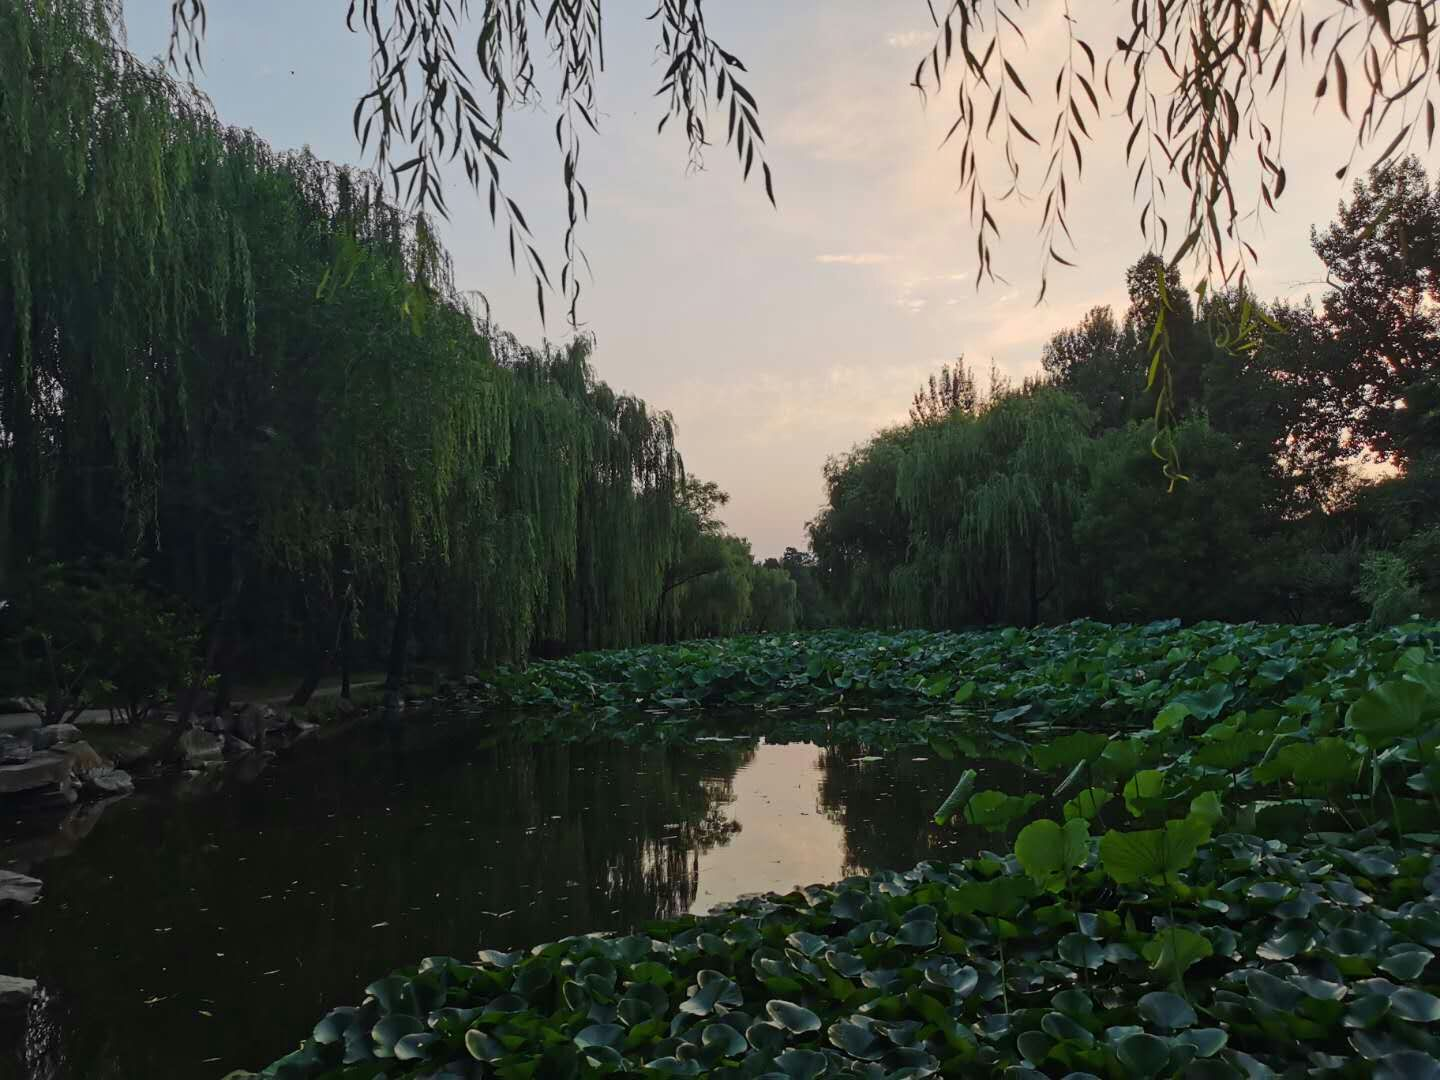
\includegraphics[width=\linewidth]{figures/暮中荷塘.jpg}
	暮中荷塘
\end{figure}

相传荷塘的荷花不是普通的荷花,而是通过美貌与幻音蛊惑行人的荷仙。
白日里,荷塘和其他的莲池并没有什么不同的地方,水面一片清圆,莲花亭亭玉立于碧叶之间,粉嫩白皙,宛若下凡的仙女,妩媚却又神圣。
但当夜色降临,时间逐渐逼近午夜,本应渐归沉寂的荷塘又会热闹起来,一朵朵莲花竟化作了美丽的舞女,荷仙的午夜晚会开始了。
她们的歌声带有魔力,恰如希腊神话中的塞壬,迷人心魂,听者皆会在不知不觉间进入幻境。
她们身形曼妙,舞姿绰约,月色中,树影下,光影迷幻,仿佛梵婀玲上婉转奏着的名曲。
若是恰逢水面上升腾起些许雾气,远远望去,舞池如同隔了一层薄纱,仙子们的身影更加朦胧。醉心观赏时,恍若在悄悄欣赏着远方高楼上渺茫的歌声,逐渐陶醉其中。神游中更好像嗅到了仙子们身上独有的莲香,撩拨着观众的欲望。

本来,我们或许永远都不会知道,在这荷塘中还有这样的聚会。
但是90多年前,一位正处在迷茫中的学者,恰在夜间散步时误入了此地。沉醉在荷仙的歌声与舞蹈中,他很快陷入了神游。在恍惚间他已远离了荷塘,很快回到了自己门前。
从荷塘脱身后,他提笔记下此事,人们才初次了解到,在荷塘还有这样一个不属于人类的世界。

并不是每一个在午夜到过荷塘的人都能如此幸运地全身而退。
这位学者到访的那晚,正值满月,透过薄云,朦胧的月色实在美妙,荷仙们心情正好,或许正是因此,仙子们并没有为难于他。
然而月有阴晴圆缺,据说当月光彻底被云遮住或是恰逢朔月之时,仙子的舞池失去了光源,黑暗中舞会难以举办,烦躁的荷仙便会借路过此地而打扰了聚会的路人撒气,吸其精气,啖其血肉,啮其骨髓。
而我们去寻零零阁的那晚,即醉酒男子进入的那晚,恰是五月初三,又是阴天,本就晦暗的如钩月彻底挡在了阴云之后,是个真正的月黑杀人夜。
想到这里,我们不禁生出了一身冷汗,叹息那醉酒男子的同时,也暗自庆幸,自己没有在池边徘徊,上山寻得阁子后便及时下山离开,脱得险地。

\vfill

\paragraph{附注}
本章故事的创意,皆启发、化用自朱自清先生的《荷塘月色》。
